\cleardoublepage\chapter{Fundamentals and Related Work}\label{sec:sota}

\section{Event-based cameras}

Event cameras ~\cite{gallego2020} are bio-inspired sensors that differ from conventional frame cameras, as instead of capturing images at a fixed rate specified by an external clock (e.g. 30 fps), they asynchronously measure per-pixel brightness changes, and output a stream of events that encode the time, location and sign of the brightness changes.\\

These novel cameras offer attractive properties compared to traditional cameras:

\begin{itemize}
	\item High temporal resolution: events are detected and timestamped with microsecond resolution. Therefore, event cameras can capture very fast motions, without suffering from motion blur, typical of frame-based cameras.
	\item Low latency: each pixel works independently, thus as soon as the change is detected, it is transmitted. This working principle enables event cameras to have minimal latency, e.g. about 10 $\mu$s on the lab bench, and sub-millisecond in the real world.
	\item High Dynamic Range (HDR): the range for event cameras exceeds 120 dB, in comparison to the 60 dB of high-quality, frame-based cameras, making them able to acquire information in challenging illumination conditions.
	\item Low power consumption: as event cameras transmit only brightness changes, removing redundant data, power is only used to process changing pixels, e.g., at the die level, most cameras use about 10 mW.
\end{itemize}

Hence, event cameras have a large potential for robotics and computer vision in challenging scenarios for traditional cameras. Concretely, it is really suitable for highly responsive systems, like manipulation tasks, where a fast perception is required. Actually, the speed advantage of event-based cameras to enable fast closed-loop control has been demonstrated in ~\cite{CL1}, ~\cite{CL2}, ~\cite{CL3}, ~\cite{CL4}. Such low perception latencies provide enough time to respond effectively, for example, to balance a pencil on its tip.\\

This is why, event-based cameras can be an appropriate choice of visual sensor to perform a corrective actions in robot manipulation. However, novel methods are required to process the unconventional output of these sensors in order to unlock their potential. In ~\cite{gallego2020}, a comprehensive overview of the emerging field of event-based vision is provided.

\section{Robotic arms}

A robotic arm is a type of mechanical arm that is programmed to execute a specific task or job quickly, efficiently and extremely accurately. The links of such manipulator are connected generally by motor-driven joints, which allow either rotational motion or translational displacement. These links form a kinematic chain, trying to resemble the functionality of a human arm, where the main joints imitate the shoulder, elbow and wrist. Moreover, end-effectors are devices that are attached to end of a robotic arm and are in charge to interact with the environment, similarly as a human hand would do.\\

These kind of robots are widely used in industrial applications as they are ideal for operations which are repetitive, consistent and require a very high degree of accuracy, as well as for applications in which a human worker might struggle to perform safely. Concretely, articulated robots are the most common types of industrial robots and they consist of at least three rotary joints. In addition, collaborative robots, or cobots, are designed to work in collaboration with humans, presenting lightweight materials, rounded edges, limited speed and force, and sensors combined with software that ensure safe behavior.\\

A robotic arm is characterized mainly by the:

\begin{itemize}
	\item Degrees of Freedom (DoF): number of independent motions in which the end-effector can move, defined by the number of axes of motion of the manipulator. For example, a human arm has seven DoF.
	\item Work envelope: a three-dimensional shape that defines the boundaries that the robot manipulator can reach.
	\item Payload: the maximum payload is the amount of weight carried by the robot manipulator at reduced speed while maintaining rated precision. Nominal payload is measured at maximum speed while maintaining rated precision. These ratings are highly dependent on the size and shape of the payload. 
\end{itemize}

As mentioned, the links in a robotic arm form a kinematic chain, where each joint is controlled by servomotors. For articulated robots, according to the angular position of each joint, the end-effector ends up being in a certain pose, which can be computed using the forward kinematics. However, usually the end-effector's pose is imposed and the controller needs to set the angular positions of the joints, which are obtained using the inverse kinematics of the mechanism.

\section{Related Work}

Prior work on event-based cameras has demonstrated the outstanding capabilities of these sensors for object tracking ~\cite{OT1}, ~\cite{OT2}, ~\cite{gallego2020} and ego-motion estimation ~\cite{EM1}, ~\cite{EM2}, ~\cite{gallego2020}. However, little work has been done on event-based perception for in-hand object tracking and robot manipulation. The scarce literature in the topic is due to the fact that event-based cameras are an emerging technology, still in prototype phase (commercially available only since 2008), and they are costly (thousand USDs) compared to traditional frame-based cameras. Additionally, there is an entry barrier for people to get familiarized with the remarkably different sensing modality and the type of output produced by event-based cameras.\\

In ~\cite{barranco2018} an event-based camera was used as end-effector of a robot arm to acquire data for visual tracking, but not for manipulation. Instead \cite{muthusamy2020} presents a visual servoing method using an event camera and a switching control strategy to explore, reach and grasp an object, in order to complete a manipulation task. However, they only use simple, high-contrast objects (a white cardboard triangle or rectangle). Moreover, ~\cite{huang2021} proposes an event-based robotic grasping framework for multiple known and unknown objects in a cluttered scene, but only providing a fix plan to be executed and not detecting slip or failure during the grasping operation.\\

In terms of slip detection, ~\cite{rigi2018} proposes a novel approach to detect incipient slip according to the contact area between a transparent silicone medium and different objects, using an event-based camera. The experimental setup consists of the robot arm, event-based camera, LED, silicone medium and adjustable camera frame, as depicted in ~\Cref{fig:rigi2018}. Moreover, the high-speed camera is used for validation purposes. In the experiments, the robot arm applies a force to an object perpendicularly to the surface of the silicon medium and afterwards the force from the robot arm was gradually reduced to release the object, in order to induce slip. This approach is not suitable for pick-and-place operations, where the slip occurs during the moving phase and not pushing the object against a deformable medium. Also, the sensor consists of the event-based camera, LED, silicone medium and adjustable camera frame, which are used in a static way, and in our pick-and-place scenario they would have to move attached to the robot, being prone to vibrations.\\

\begin{figure}[h]
    \centering
    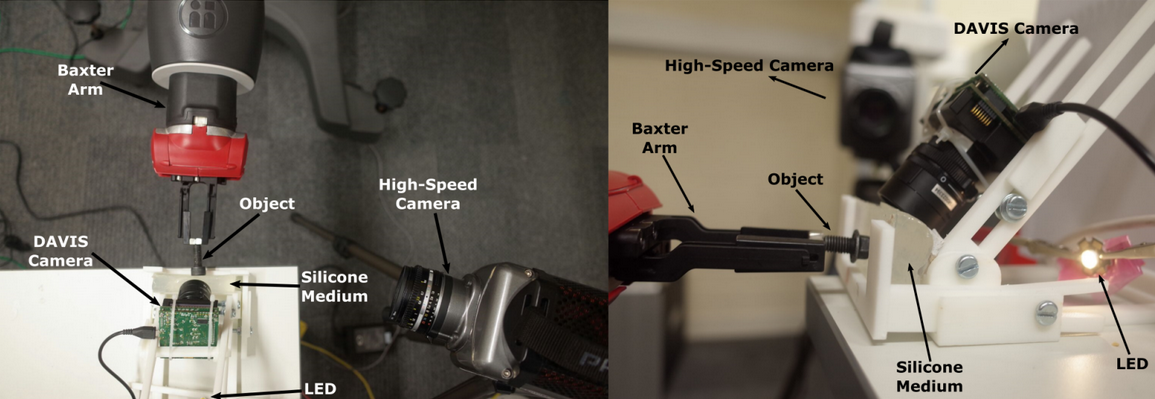
\includegraphics[width=\textwidth]{resources/images/rigi2018}
    \caption{Top-down (left) and sideways (right) views of the experiment setup ~\cite{rigi2018}.}\label{fig:rigi2018}
\end{figure}

Muthusamy et al. \cite{muthusamy2020slip} presents a first study on using an event-based camera with narrow field of view to detect slip during manipulation, but it analyzes only tiny motions. Moreover, it provides a slip suppression strategy regulating the grip force. The experimental setup is formed by the Baxter robot, electric parallel gripper, F/T sensor and a finger with an integrated event-based camera, as shown in ~\Cref{fig:muthusamy2020slip}. The F/T sensor measures six components of force and torque and is used only for validation purposes. In terms of the event-based camera, it observes the object through one of the transparent fingers of the gripper, which limits the information available from the object. The sensor itself moves attached to the gripper in this case, being suitable for pick-and-place operations.

\begin{figure}[h]
    \centering
    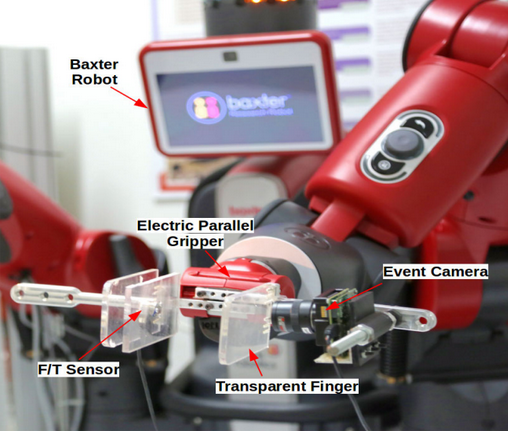
\includegraphics[width=0.7\textwidth]{resources/images/muthusamy2020slip}
    \caption{Experiment setup: Baxter Gripper with event-based finger prototype ~\cite{muthusamy2020slip}.}\label{fig:muthusamy2020slip}
\end{figure}

Another family of sensors widely used in the literature for slip detection are the tactile sensors, which may provide physical signals like the ratio of shear force to normal force, vibration or acceleration. In ~\cite{gelsight2017}, a tactile sensor, called GelSight sensor, is used for measuring geometry and detecting slip. Concretely, both translational and rotational slips are considered during grasp tasks, not complete pick-and-place operations. The GelSight sensor detects slip based on 3 major clues: the relative displacement between the objects and the sensor surface, the shear displacement distribution of the markers on the sensor surface and the change in the contact
area. They perform grasp experiments on 37 daily-use objects, lifting these slowly for 3 cm and then stopping. Each object is lifted 7 to 10 times, with different gripper forces, and the data is manually labeled indicating whether a slip occurred or not during the grasping and lifting process. Moreover, they implement a grasp closed-loop control with the feedback of the GelSight slip detection, using 33 objects and grasping each of them 3 times. If slip is detected the object is released and it is re-grasped with a higher gripping force.\\

In ~\cite{gelsight2018} the tactile information obtained from the GelSight sensor is combined with visual information coming from an external camera (standard webcam). The new setup including this camera is depicted in ~\Cref{fig:gelsight}. In this case a dataset is created including more than 1200 grasp experiments with 94 objects in total (for the train and test sets) and a deep neural network is trained to classify whether in a certain lifting sequence a slip has occured or not. These lifting sequences consider only small vertical motions with a non-textured (uniform) background and, in each grasp, the gripper width is modified in order to provoke slip or even complete failure in the grasp, which is manually annotated. They conclude that the best results are achieved combining tactile and vision information and, when using only vision information, much better results are achieved when the difference of images are taken into account, instead of the raw images. Note that using difference of images coming from a standard camera is a similar paradigm compared to event-based cameras, but these present a lower latency and therefore the feedback is faster.

\begin{figure}[h]
    \centering
    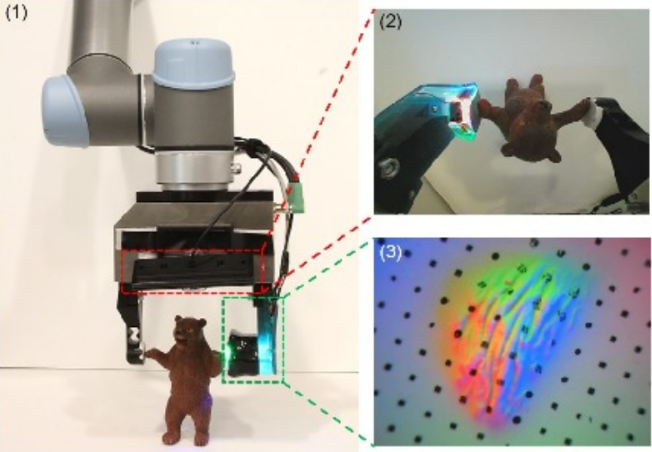
\includegraphics[width=0.7\textwidth]{resources/images/gelsight}
    \caption{(1) Experiment setup: UR5 robot arm with gripper, GelSight sensor and external camera. (2) Image captured by the external camera. (3) Image from GelSight sensor ~\cite{gelsight2018}.}\label{fig:gelsight}
\end{figure}

More work has been done in the combination of tactile and visual information, as in ~\cite{rss2020}, where they designed a Visual-Tactile Spiking Neural Network for rotational slip detection using their NeuTouch tactile sensor and the Prophesee event camera. In the experimental setup, see ~\Cref{fig:rss2020}, they also include 2 RGB cameras (for visualization and validation purposes), one mounted on the end-effector pointing towards the griper and the second one was placed to provide a view of the scene, and 11 OptiTrack cameras were used to collect ground-truth data. OptiTrack is a motion capture system that tracks the motion of some reflective markers attached to, in this case, the end-effector and the object. With this information the relative trajectory of the object with respect to the end-effector can be analyzed to determine whether the slip occurred or not. During the experiments they used a object built with Lego Duplo blocks with hidden masses. One variant was designed to be balanced at the grasp point and the second one, modifying the hidden masses, is unstable to induce rotational slip. Both variants are lifted by 10 cm off the table (in 0.75 s) and then holded, repeating this 50 times for each variant. However, the model was trained only during the first 0.15 s of the lifting phase, as they focus on early slip detection. Additionally, the background scene recorded by the cameras corresponds to a controlled black background.

\begin{figure}[h]
    \centering
    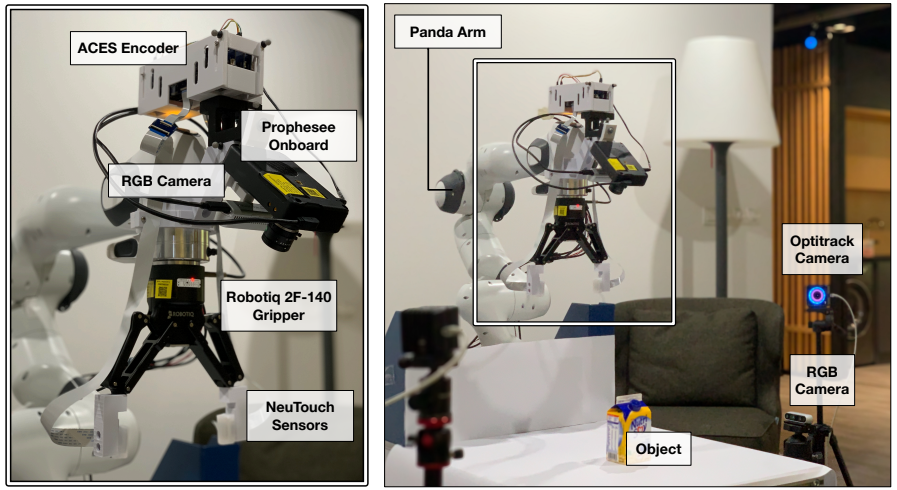
\includegraphics[width=0.95\textwidth]{resources/images/rss2020}
    \caption{Experiment setup: Robot arm, Prophesee event camera, Robotiq gripper, NeuTouch sensors, RGB and OptiTrack cameras ~\cite{rss2020}.}\label{fig:rss2020}
\end{figure}

\section{Conclusion}

Robot arms are widely used for pick-and-place motions and, combined with event-based cameras, which present several advantages compared to conventional frame cameras, they have the potential to form a robust manipulation and slip detection framework.\\

Even though there is some literature tackling this issue, none of them are considering the whole pick-and-place motion to detect slip and instead they are just analyzing tiny motions. Moreover, to make sure the solution generalizes the dataset should also include daily use objects and non-controlled background. When it comes to label the samples, some of the works determine if there is a slip or not by human inspection, however, ideally, having ground-truth data would be more suitable.\\

Most recent works are focusing on combining tactile and vision information, however, in industrial applications tactile sensors may have disadvantages like wear and a lack of long-term robustness. So, considering only visual information, concretely coming from an event-based camera, the placement of the camera in the end-effector should ensure a wide field of view, like in ~\cite{gelsight2018} and ~\cite{rss2020}.\\

In short, the topic of event-based vision for robot manipulation remains largely unexplored and thus offers great opportunities.\\

After having analyzed several experimental setups regarding robot manipulation with slip detection, in the next chapter our particular experimental setup is described.
